\documentclass{article}
\usepackage[top=1in, bottom=1in, left=1in, right=1in]{geometry}
\usepackage{polski}
\usepackage[utf8]{inputenc}
\usepackage{multirow}
\usepackage{graphicx}
\usepackage{float}
\begin{document}
\title{\huge\bfseries Badanie zjawiska Halla}
\date{}
\author{}
\maketitle
\section{Wstęp teoretyczny}
\textbf{Efekt Halla} - zjawisko powstania różnicy potencjałów(napięcia) pomiędzy przeciwległymi ściankami półprzewodnika lub metalu w kierunku prostopadłym do kierunku przepływu prądu oraz kierunku wektora indukcji zewnętrznego pola magnetycznego. \\
Na ładunek elektryczny poruszający się w polu elektromagnetycznym działa \textbf{siła Lorentz'a} i wyrażana jest wzorem
$$F = qvB\sin \alpha $$
Wektor siły jest prostopadły zarówno do kierunku wektora indukcji magnetycznej i wektora prędkości.\\
\textbf{Natężenie pola magnetycznego przewodnika} jest tym większe, im większe jest natężenie prądu w przewodniku i im mniejsza jest odległość punktu pola od przewodnika. Natężenie pola magnetycznego określa się wzorem
$$H = \frac{l}{2\pi r} [\frac{A}{m}]$$
\textbf{Solenoid} to cewka powietrzna(bez rdzenia) która wytwarza jednorodne pole magnetyczne. Natężenie pola wyrażane jest wzorem
$$H = n \cdot I $$
gdzie:\\
H - natężenie pola\\
n - liczba zwojów cewki\\
I - natężenie prądu elektrycznego\\\\
\textbf{Efekt Halla umożliwia} pomiar znaku ładunków poruszających się w przewodniku oraz ich koncentrację oraz
dla znanych materiałów pozwala określić wartość indukcji pola magnetycznego.
\section{Opracowanie pomiarów}
Tabela przedstawia wyniki przeprowadzonych pomiarów:
\begin{center}
    \begin{tabular}{|c|c|c|c|c|}\hline
    \multicolumn{5}{|c|}{$U_Y, mV$} \\ \hline
    $Is,mA$ & $I = 0,000(29)A$ & $I = 1,000(40)A$ & $I = 2,000(52)A$ & $I = 3,000(64)A$ \\ \hline
$-6,000(33)$ & $-2,200(62)$ & $-0,600(70)$ & $1,100(75)$ & $2,900(80)$ \\ \hline
$-5,000(29)$ & $-1,800(61)$ & $-0,500(68)$ & $0,900(72)$ & $2,400(77)$ \\ \hline
$-4,000(24)$ & $-1,500(60)$ & $-0,400(66)$ & $0,700(69)$ & $1,900(73)$ \\ \hline
$-3,000(20)$ & $-1,100(59)$ & $-0,300(64)$ & $0,500(66)$ & $1,500(69)$ \\ \hline
$-2,000(15)$ & $-0,700(57)$ & $-0,200(62)$ & $0,300(62)$ & $1,000(63)$ \\ \hline
$-1,000(10)$ & $-0,300(56)$ & $-0,100(58)$ & $0,200(58)$ & $0,500(59)$ \\ \hline
$0,000(55)$ & $0,000(55)$ & $0,000(55)$ & $0,000(55)$ & $0,000(55)$ \\ \hline
$1,000(10)$ & $0,400(56)$ & $0,100(59)$ & $-0,100(57)$ & $-0,400(59)$ \\ \hline
$2,000(15)$ & $0,800(57)$ & $0,300(61)$ & $-0,200(60)$ & $-0,800(64)$ \\ \hline
$3,000(20)$ & $1,200(58)$ & $0,400(63)$ & $-0,400(63)$ & $-1,300(68)$ \\ \hline
$4,000(24)$ & $1,700(59)$ & $0,500(65)$ & $-0,500(66)$ & $-1,700(72)$ \\ \hline
$5,000(29)$ & $2,100(60)$ & $0,700(67)$ & $-0,600(69)$ & $-2,200(77)$ \\ \hline
$6,000(33)$ & $2,500(61)$ & $0,800(69)$ & $-0,800(72)$ & $-2,600(81)$ \\ \hline
    \end{tabular}
\end{center}
Niepewności pomiarowe zostały obliczone na podstawie wzoru
$$u_a = \frac{x}{\sqrt{3}}$$
, gdzie x to niepewność pomiarowa przedstawiona przez producenta sprzętu pomiarowego i wynosi ona następująco:
\begin{center}
$2,0\%W + 50mA$ - miliamperomierz\\
$0,8\%W + 10\mu A$ - amperomierz\\
$0,5\%W + 100\mu V$ - woltomierz
\end{center}
Od wszystkich napięć poprzecznych odjęliśmy napięcie występujące przy zerowym prądzie cewki. Wyniki ukazuje tabela:
\begin{center}
    \begin{tabular}{|c|c|c|}\hline
$U_{H1}=U1-U0, V$ & $U_{H2}=U2-U0, V$ & $U_{H3}=U3-U0, V$ \\ \hline
$I = 1A$ & $I = 2A$ & $I = 3A$ \\ \hline 
$0,001600(95)$ & $0,003300(98)$ & $0,005100(11)$ \\ \hline
$0,001300(93)$ & $0,002700(94)$ & $0,004200(99)$ \\ \hline
$0,001100(91)$ & $0,002200(91)$ & $0,003400(96)$ \\ \hline
$0,000800(89)$ & $0,001600(89)$ & $0,002600(93)$ \\ \hline
$0,000500(87)$ & $0,001000(87)$ & $0,001700(90)$ \\ \hline
$0,000200(85)$ & $0,000500(85)$ & $0,000800(87)$ \\ \hline
$0,000000(83)$ & $0,000000(83)$ & $0,000000(83)$ \\ \hline
$-0,000300(85)$ & $-0,000500(86)$ & $-0,000800(86)$ \\ \hline
$-0,000500(87)$ & $-0,001000(89)$ & $-0,001600(89)$ \\ \hline
$-0,000800(89)$ & $-0,001600(92)$ & $-0,002500(93)$ \\ \hline
$-0,001200(91)$ & $-0,002200(95)$ & $-0,003400(95)$ \\ \hline
$-0,001400(93)$ & $-0,002700(97)$ & $-0,004300(98)$ \\ \hline
$-0,001700(94)$ & $-0,003300(99)$ & $-0,005100(10)$ \\ \hline
    \end{tabular}
\end{center}
Niepewność obliczona ze wzoru:
$$u(U_H) = \sqrt{(u(U_Y))^2+(u(U_Y0))^2}$$
Na wykresie(1) przedstawiliśmy zależności napięcia Halla $U_H$ w funkcji natężenia prądu sterującego $I_S$\\
Następnie zestawiliśmy współczynniki kierunkowe otrzymanych charakterystyk. Ukazuje je tabela:
\begin{center}
    \begin{tabular}{|c|c|c|}\hline
$I = 1A$ & $I = 2A$ & $I = 3A$ \\ \hline 
$-0,2736(39)$ & $-0,5429(41)$ & $-0,8484(45)$\\ \hline
    \end{tabular}
\end{center}
Wzór na stałą Halla $R_H$:
$$R_H = \frac{d\cdot U_H}{A\cdot I_s \cdot I}$$
,gdzie \\
$A=0,0045$\\
$d=0,0815(50)mm$\\
I przekształcając go na współczynnik $a$ otrzymujemy
$$a = \frac{AR_HI}{d}$$
$$R_H = \frac{ad}{AI}$$
$$R_H = \frac{0,2736 \cdot 0,0016}{0,0045 \cdot -6 \cdot 1} = -4,9552$$
\begin{center}
    \begin{tabular}{|c|c|c|}\hline 
    \multicolumn{3}{|c|}{$R_H$} \\ \hline
     $I = 1A$ & $I = 2A$ & $I = 3A$ \\ \hline 
$-4,95(39)$ &  $-4,92(33)$ &  $-5,12(35)$ \\ \hline
    \end{tabular}
\end{center}
Rachunek jednostek:
$$\frac{mV}{AT}=\frac{m}{A} \cdot \frac{As^2m^2kg}{As^3kg} = \frac{m^3}{As} = \frac{m^3}{C}$$
Niepewność obliczyliśmy wykorzystując prawo przenoszenia niepewności:
$$u(R_H) = \sqrt{(\frac{d}{AI}u(a))^2 + (\frac{a}{AI}u(d))^2 + (\frac{-ad}{AI^2}u(I))^2}$$
Srednia ważona i jej niepewność zostały obliczone ze wzorów
$$\frac{\Sigma \omega_i \phi_i}{\Sigma \phi_i}$$
,gdzie $\phi$ to waga obliczonej wartości obliczaną wzorem
$$\phi = \frac{1}{u(R_H)^2}$$
a $\omega$ to wartości $R_H$\\
Niepewność średniej ważonej obliczyliśmy z
$$\frac{1}{\sqrt{\Sigma \phi_i}}$$
Więc średnia ważona obliczanej wartości wynosi
$$R_{Hsr} = -4,95(24) \frac{m^3}{C}$$
Ze wzoru obliczyliśmy czułość hallotronu
$$\gamma_0= \frac{a}{AI}$$
\begin{center}
    \begin{tabular}{|c|c|c|}\hline 
    \multicolumn{3}{|c|}{$\gamma, \frac{V}{AT}$} \\ \hline
     $a_1 = -0,2736$ & $a_2 = -0,5429$ & $a_3 = -0,8484$ \\ \hline 
$-60,80(39)$ &  $-60,32(33)$ &  $-62,84(35)$ \\ \hline
    \end{tabular}
\end{center}
Niepewność wyliczyliśmy propagacją niepewności
$$\sqrt{(\frac{1}{AI}u(a))^2 + (\frac{-a}{AI^2}u(I))^2}$$
Obliczyliśmy średnią ważoną czułości
$$\gamma_{sr} = -61,23(1,54) \frac{V}{AT}$$
\section{Wnioski}
Zbadane przez nas napęcie poprzeczne pozwoliło nam wyznaczyć stałą Halla. Wartość średnia obliczonej przez nas stałej Halla jest ujemna co świadczy o tym, że w układzie został zastosowany półprzewodnik typu n(domieszkowany).
\begin{figure}[ht]
\caption{Wykres}
\centering
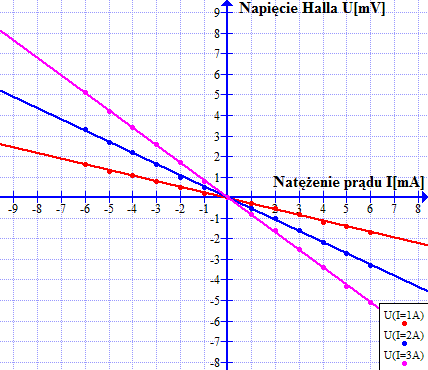
\includegraphics{wykres_1.png}
\end{figure}\\
\end{document}